%%\section{Топологические пространства}
%\subsection{Основное определение}
\section{\centering Некоторые сведения из топологии}
Здесь будут приведены некоторые теоретические сведения из топологии, используемые в дальнейшем. Более подробно об этом можно прочитать в специальной литературе, например в \cite{Viro, Vick, Hatcher}.%, \cite{Vick}, \cite{Hatcher}.

Основным объектом в топологическом анализе данных можно считать симплициальный комплекс. В некотором смысле, это обобщение графов на более старшие размерности. В частности, по любому графу можно построить (флаговый) комплекс, объявив каждую его клику симплексом.

Симплексом размерности $n$ называют Выпуклую оболочку набора $\{ x_0, ..., x_n \} \subset \mathbb{R}^d$, причем такого, что векторы $ x_1 - x_0, ..., x_n - x_0 $ линейно независимы. Гранью $n$-симплекса называют $k$-симплекс, который получается как выпуклая оболочка некоторого подмножества вершин этого симплекса.

%Выпуклую оболочку набора $\{ x_0, ..., x_n \} \subset \mathbb{R}^d$, причем такого, что векторы $ x_1 - x_0, ..., x_n - x_0 $ линейно независимы, называют $n$-мерным симплексом. Гранью $n$-симплекса называют $k$-симплекс, который получается как выпуклая оболочка некоторого подмножества вершин этого симплекса.

Так, $n$-симплекс можно рассматривать как $n$-мерное обобщение треугольника и тетраэдра. На рисунке \ref{simplex} приведены примеры симплексов.
\begin{figure}[!htbp]
	\centering
	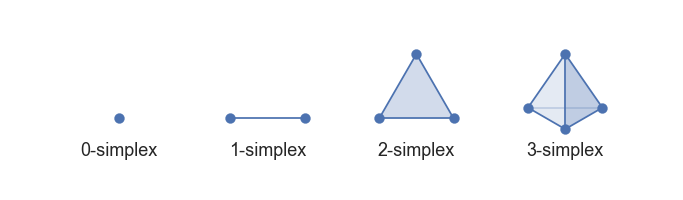
\includegraphics[width=0.5\linewidth, keepaspectratio=true]{simplices.png}
	\caption{Различные симплексы}
	\label{simplex}
\end{figure}
\begin{definition}
	Топологический симплициальный комплекс $K$ -- это множество симплексов такое, что:
	\begin{enumerate}
		\item Для каждого симплекса из $K$ его грани тоже лежат в $K$.
		\item Пересечение любых двух симплексов $\sigma, \tau \in K$ либо пусто, либо является гранью и $\sigma$, и $\tau$.
	\end{enumerate}
\end{definition}
На рисунке \ref{simplicial_complex} представлен пример симплициального комплекса. Так как среди всех симплексов, входящих в представленный на рисунке комплекс, размерность не выше $3$, то и размерность симплициального комплекса равна $3$.
\begin{figure}[!htbp]
	\centering
	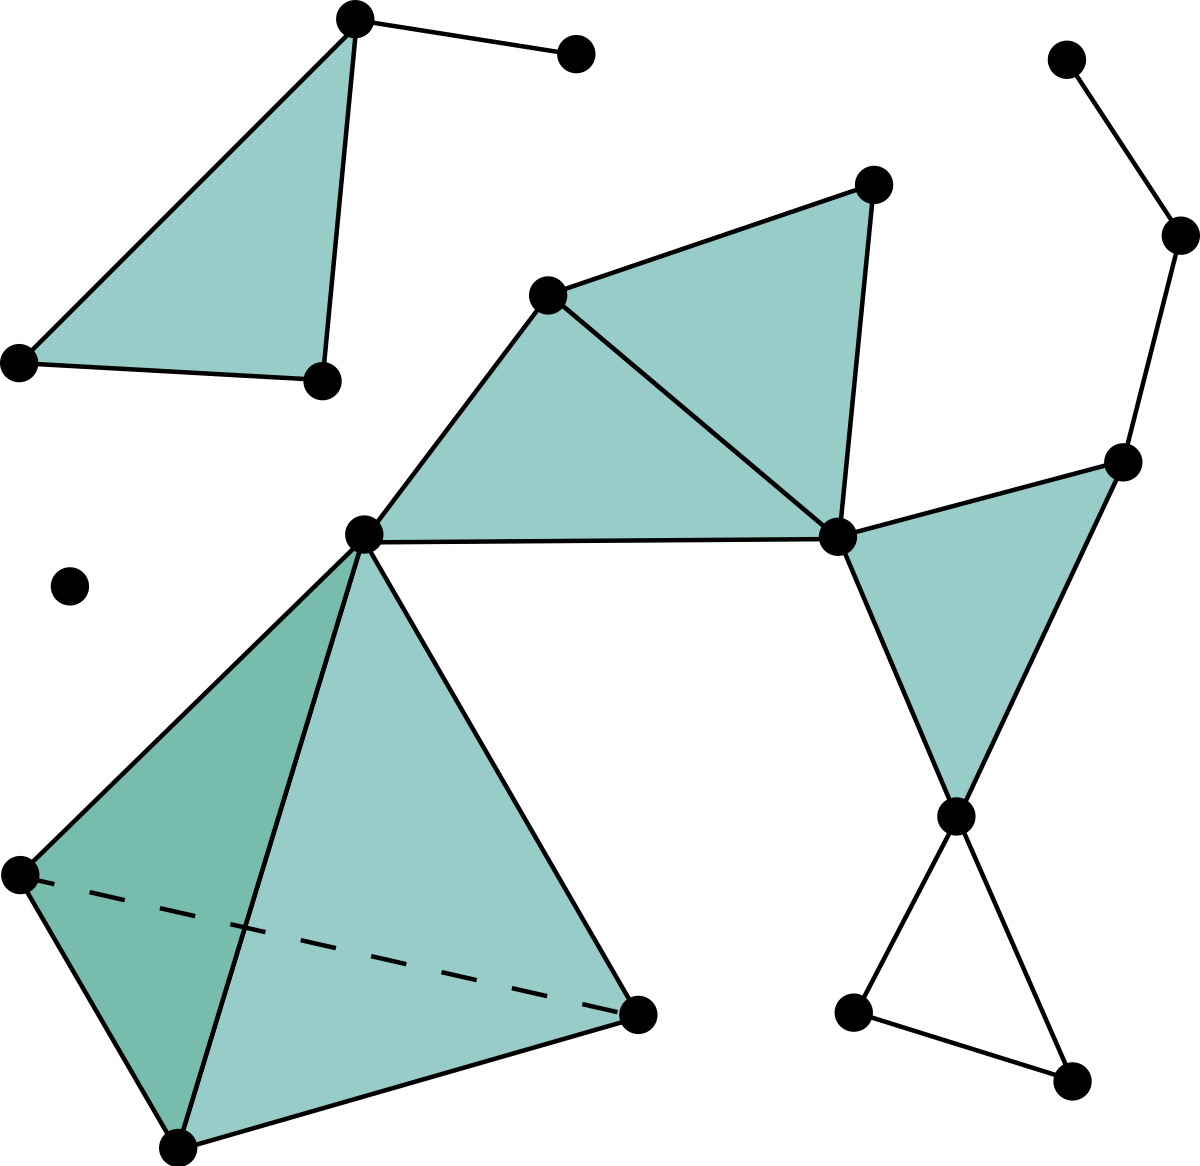
\includegraphics[width=0.5\linewidth, keepaspectratio=true]{simplicial_complex.png}
	\caption{Симплициальный комплекс}
	\label{simplicial_complex}
\end{figure}
По топологическому симплициальному комплексу можно построить топологическое пространство -- объединение его симплексов. Такие пространства тоже называют симплициальными комплексами. В таком пространстве топология индуцируется топологией на $\mathbb{R}^d$.

Имея топологическое пространство $X$, говорят, что набор его подмножеств $\{U_i : i \in J\} $ является {\it покрытием}, если $ \bigcup\limits_{i \in J} U_i = X$. Покрытие называется {\it открытым}, если оно состоит из открытых множеств.

По покрытию пространства можно построить нерв покрытия  (рисунке. \ref{nerve}) -- симплициальный комплекс, соответствующий топологическому пространству и имеющий различные интересные топологические свойства. Пусть $ [m] \coloneqq \{1, ..., m\} $ -- $m$-элементное множество.
\begin{definition}
	Нерв покрытия $N(U)$, соответствующий топологическому пространству $X$, -- это абстрактный симплициальный комплекс на $[m]$, такой что $ \{k_1, ..., k_s\} \in N(U) $ если $ U_{k_1} \cap ... \cap U_{k_s} \neq \emptyset $.
\end{definition}
\begin{figure}[h!]
	\begin{center}
		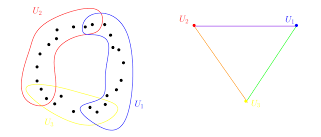
\includegraphics[width=0.75\textwidth]{nerve.png}\\
		\caption{Покрытие пространства и нерв покрытия}
		\label{nerve}
	\end{center}
\end{figure}
Если имеется 2 непрерывных отображения $f, g : X \to Y$, то говорят, что $f$ {\it гомотопно} $g$, если существует такое отображение ${H: X\times I \to Y}$, что ${H(x,0) = f}$ и ${H(x,1) = g}$. В таких случаях пишут, что ${f \sim g}$. Гомотопия является отношением эквивалентности на множестве непрерывных отображений ${ C(X,Y) }$.


Два топологических пространства $X,Y$ гомотопически эквивалентны (${X \sim Y}$), если существует такая пара ${(f,g) \in C(X,Y)^2}$, такая, что ${f \circ g \sim id_Y}$ и ${g \circ f \sim id_X}$.

С понятием нерва покрытия связана очень важная лемма:
\begin{lemma*}[о нерве]
	Если $U$ -- открытое покрытие, такое, что любое пересечение его подмножеств либо пусто, либо гомотопически эквивалентно точке, то нерв покрытия пространства $X$ гомотопически эквивалентен самому пространству
	\[ \forall I \in N(U) \left( \bigcap\limits_{i \in I} U_i = \emptyset \lor \bigcap\limits_{i \in I} U_i \sim pt \rightarrow N(U) \sim X \right). \]
\end{lemma*}

Как всякая хорошая математическая структура, симплициальные комплексы образуют {\it категорию} \cat{SCpx}. Морфизмами в такой категории являются симплициальные отображения $\varphi : M \to N$, т.е. такие отображения, что для каждого симплекса из $M$ $\varphi$ является линейным отображением на симплекс из $N$. 

Имея симплициальный комплекс, можно найти его симплициальные гомологии. Такие гомологии можно рассматривать как функтор из категории симплициальных комплексов в категорию абелевых групп: каждому симплициальному комплексу сопоставляется некоторая абелева группа. Замечательный момент заключается в том, что гомеоморфные симплициальные комплексы имеют одинаковые группы гомологий, а потому теория гомологий является очень удобным инструментом для изучения симплициальных комплексов. На самом деле данные утверждения можно легко обобщить на общий случай топологических пространств.

Дадим формальное определение симплициальным гомологиям. Итак, пусть $K$ -- симплициальный комплекс и $k\geq0$. 

{\it Группой $k\text{-цепей } C_k(K)$ симплициального комплекса $K$} называют (свободную абелеву) группу, элементами которого являются формальные суммы $k\text{-симплексов } K$, то есть
\[
c = \sum\limits_{i}\varepsilon_i\sigma_i,\;\; \varepsilon_i \in \mathbb{Z},
\] 
где конечное число $\varepsilon_i \neq 0$, $\sigma_i$ -- $k$-симплекс.
{\it Границей} $k$-цепи $\sum\limits_{i}\varepsilon_i\sigma_i$ называют $(k-1)$-цепь
\[
\partial_k(\sigma) = \sum\limits_{j=0}^{k}(-1)^j\sum\limits_{i}\varepsilon_i\partial_j\sigma_i,
\]
где $\partial_j\sigma_i = \partial_j [v_0, ..., v_k] = [v_0, ..., \hat{v_j}, ..., v_k] $ -- $(k-1)$-симплекс, порожденный всеми вершинами, кроме вершины $v_j$. Гомоморфизм $\partial_k : C_k(K) \to C_{k-1}(K)$ называют {\it граничным оператором}. Он удовлетворяет следующему свойству:
\[
\partial_{k-1} \circ \partial_k = 0.
\]	
То есть $ \im \partial_{k+1} \leq \ker \partial_k \leq C_k(K)$. Последовательность $C_k(K)$ и $\partial_k$ называется {\it цепным комплексом}

\begin{center}
	\begin{tikzcd}[cells={nodes={minimum height=2em}}]
	... \arrow[r, "\partial_{k+2}"] & C_{k+1} \arrow[r,"\partial_{k+1}"]  &  C_k \arrow[r,"\partial_k"] &  C_{k-1} \arrow[r, "\partial_{k-1}"] & ... \arrow[r, "\partial_1"] & C_0.
	\end{tikzcd}
\end{center}

Цепной комплекс можно визуализировать следующим образом (рисунок \ref{chain}).

\begin{figure}[!htbp]
	\centering
	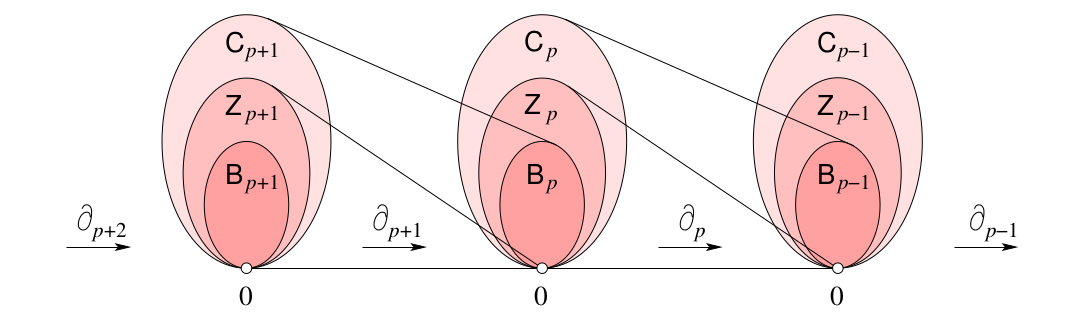
\includegraphics[width=0.5\linewidth, keepaspectratio=true]{chain.png}
	\caption{Цепной комплекс}
	\label{chain}
\end{figure}

\begin{definition}
	$k$-ой группой гомологий симплициального комплекса $K$ называют следующее фактор-пространство:
	\[
	H_k(K) = \quotient{\ker \partial_k}{\im \partial_{k+1}}.
	\]
	
	Тогда $k$-ое число Бетти -- размерность $k$-ой группы гомологий: 
	\[\beta_k(K) = \dim H_k(K).\] 
\end{definition}

При $k=0$ число Бетти описывает количество компонент связности данного пространства. При $k=1$ -- количество циклов. При $k=2$ число Бетти описывает количество  <<полостей>>. В таблице \ref{tabl:betti} представлены первые числа Бетти для некоторых пространств.

\begin{center}
	\begin{table}[!htbp]
		\centering
		\caption{Первые числа Бетти для некоторых пространств}
		\begin{tabular}{ |c|c c c| }
			\hline
			Пространство & $\beta_0$ & $\beta_1$ & $\beta_2$ \\ 
			\hline
			Pt & 1 & 0 & 0 \\ 
			$D^2$ & 1 & 0 & 0 \\ 
			Треугольник & 1 & 0 & 0 \\
			Граница треугольника & 1 & 1 & 0 \\
			$S^1$ & 1 & 1 & 0 \\
			$S^2$ & 1 & 0 & 1 \\
			$\mathbb{T}^2 = S^1 \times S^1$ & 1 & 2 & 1 \\
			\hline
		\end{tabular}
		\label{tabl:betti}
	\end{table}
\end{center}
